%% ****** Start of file aiptemplate.tex ****** %
%%
%%   This file is part of the files in the distribution of AIP substyles for REVTeX4.
%%   Version 4.1 of 9 October 2009.
%%
%
% This is a template for producing documents for use with 
% the REVTEX 4.1 document class and the AIP substyles.
% 
% Copy this file to another name and then work on that file.
% That way, you always have this original template file to use.

%\documentclass[aip,graphicx]{revtex4-1}
%\documentclass[aip,reprint]{revtex4-1}

%\usepackage{graphicx}

%\draft % marks overfull lines with a black rule on the right
%\documentclass[pre,aps,floatfix,authordate1-4,twocolumn]{revtex4-1}
%\documentclass[pre,aps,floatfix,authordate1-4]{revtex4-1}

\documentclass[aps,prl,superscriptaddress,twocolumn]{revtex4}



%\documentclass[aps,prl,preprint,groupedaddress]{revtex4}

\usepackage{rotating} 
\usepackage{times}
\usepackage{graphicx}
\usepackage{setspace}
\usepackage{amsmath}
\usepackage{epstopdf}
\usepackage[obeyFinal]{easy-todo}
\usepackage{csquotes}

\begin{document}

% Use the \preprint command to place your local institutional report number 
% on the title page in preprint mode.
% Multiple \preprint commands are allowed.
%\preprint{}

\title{NMRlipids IV: Headgroup \& glycerol backbone structures, and cation binding in bilayers with PS lipids} %Title of paper

% repeat the \author .. \affiliation  etc. as needed
% \email, \thanks, \homepage, \altaffiliation all apply to the current author.
% Explanatory text should go in the []'s, 
% actual e-mail address or url should go in the {}'s for \email and \homepage.
% Please use the appropriate macro for the type of information

% \affiliation command applies to all authors since the last \affiliation command. 
% The \affiliation command should follow the other information.

\author{O. H. Samuli Ollila}
\email[]{samuli.ollila@helsinki.fi}
%\homepage[]{Your web page}
\affiliation{Institute of Organic Chemistry and Biochemistry,
Academy of Sciences of the Czech Republic, 
Prague 6, Czech Republic}
\affiliation{Institute of Biotechnology, University of Helsinki}


% Collaboration name, if desired (requires use of superscriptaddress option in \documentclass). 
% \noaffiliation is required (may also be used with the \author command).
%\collaboration{}
%\noaffiliation

\date{\today}

\begin{abstract}
% insert abstract here
  Primarily measured but also simulated NMR order parameters will be collected also for other than phophatidylcholine
  (these are discussed in NMRlipids I) headgroup. The information will be used to understand structural differences between 
  different lipid molecules in bilayers.
\end{abstract}

%\pacs{}% insert suggested PACS numbers in braces on next line

\maketitle %\maketitle must follow title, authors, abstract and \pacs

% Body of paper goes here. Use proper sectioning commands. 
% References should be done using the \cite, \ref, and \label commands


%\label{}
\section{Introduction}

In NMRlipids I and II project we were looking for a MD model
which would correctly reproduce headgroup and glycerol
backbone structures and cation binding for PC lipid bilayers \cite{botan15,catte16}.
Here we extend the same goal for lipids with negatively charged PS headgroup.
Chemical structure of PS headgroup together with other common biological
lipids is shown in Fig. \ref{lipids}.
\begin{figure}[]
  \centering
  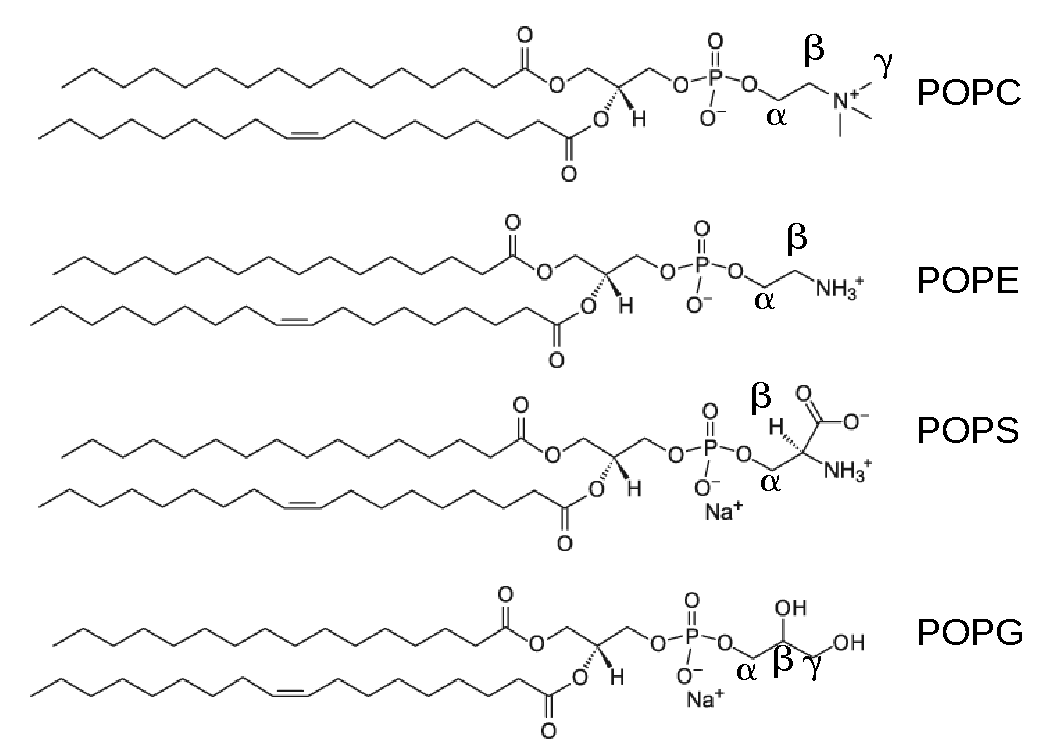
\includegraphics[width=9.0cm]{../Figs/lipids.pdf}
  \caption{\label{lipids}
    Chemical structures and labels for the headgroup carbons.
  }
\end{figure}

Absolute values of experimental order parameters for different lipid headgroups are
collected from the literature in Fig. \ref{HGorderParameters}. Since order parameter
signs are known only for PC, only absolute values are shown.
Main conclusions regarding the structure of different common lipid headgroups in the literature are \\
1) glycerol backbone structures are largely similar irrespectively of the headroup \cite{gally81}, \\
2) glycerol backbone and headgroup structure and behaviour are similar in model membranes and in bacteria \cite{gally81,scherer87,seelig90}, \\
3) headgroup structures are similar in PC, PE and PG lipids, while headgroup is more rigid in PS lipids \cite{wohlgemuth80,buldt81}. \\
Careful discussion and analysis of structural details of PE, PG or PS headgroups is not available, 
in contrast to PC lipids (see \cite{botan15} and references therein).
\begin{figure}[]
  \centering
  \includegraphics[width=9.0cm]{../Figs/HGorderparameters.eps}
  \caption{\label{HGorderParameters}
    Absolute values of order parameters for headgroup and glycerol backbone with different headgroups
    from experiments. POPC values are from \cite{ferreira13}, DOPS from \cite{browning80} contains 0.1M of NaCl,
    POPG from \cite{borle85} contains 10nM PIPES, DPPG from \cite{wohlgemuth80} contains  10mM PIPES and 100mM NaCl,
    DPPE from \cite{seelig76}, E.coliPE and E.coliPG are from \cite{gally81}.
  }
\end{figure}

As shown in Fig. \ref{HGorderparametersPCvsPEPSPGchol}, order parameters of PC
headgroup behave in various lipid mixtures as expected from the electrometer concept \cite{seelig87, scherer87},
i.e., order parameters increase when anionic lipids are mixed with PC and decrease with cationic
surfactants. The changes with the addition of neutral lipids is significantly smaller.
\begin{figure}[]
  \centering
  \includegraphics[width=8.0cm]{../Figs/HGorderparametersPCvsPEPSPGchol.eps}
  \caption{\label{HGorderparametersPCvsPEPSPGchol}
    PC headgroup order parameters from experiments of mixtures with
    PE, PS, PG and cholesterol \cite{scherer87,scherer89,ferreira13}.
    Signs are determined as discussed in \cite{botan15,ollila16}.
  }
\end{figure}





%Phospholipids containing various polar headgroups and acyl
%chains are essential building blocks of biological membranes.
%Atomistic level structural details of lipids and lipid-ion 
%interactions are considered highly important in several
%biological processes. The lipid structure and ion binding
%can be studied in detail with NMR spectroscopy. However,
%the structural interpretation of NMR data requires usage
%of models. The combination of classical molecular dynamics
%simulations with NMR data, especially with C-H bond
%order parameters, can potentially give atomistic resolution
%interpretation of structure and dynamics of molecules \cite{botan15,ollila16,ferreira16}. 

%Our recent studies concluded that MD models are cabable to
%give structural interpretation for phosphatidylcholine 
%hydrophopic acyl chain region, while hydrophilic headgrop, glycerol 
%backbone and cation binding posed a major challenge for current
%force fields \cite{botan15,ollila16,catte16,ferreira16}. 
%These conclusions were reached by reviewing extensively 
%available experimental data from various sources and using
%NMRlipids Open Collaboration project to collect massive 
%amount of simulation data \cite{botan15,catte16}.

%Here we apply the same approach in search of MD simulation
%models which would reproduce glycerol backbone and 
%headgroup structures of lipids with PE, PG and PS headgroups.  
%In addition, we attempt to find a MD simulation model
%that would be able to correctly describe cation binding in
%bilayer containing negatively charged PG and PS lipids.


%Several MD simulation models have succesfully described 
%acyl chain structures and their qaulitative changes in different
%conditions for phosphatidylcholine lipids (for review see \cite{ollila16}).
%However, the current simulation models were not found to be accurate
%enough for full structural interpretation of phosphatidylcholine headgroup and
%glycerol backbone \cite{botan15}. Also Na$ +$  binding affinities
%were found to be significantly overestimated in several models and 
%none of the available models was able to Ca$2+$ 

%\section{Methods}

%\subsection{Molecular dynamics simulations}

\section{Results and Discussion}

\subsection{PS headgroup and glycerol backbone structure in simulations and experiments}
The headgroup order parameters of DOPS and POPS bilayers 
from different experiments and simulations are shown in
Figs. \ref{HGorderParametersPS}.
None of the tested models gives satisfactory agreement with
experiments for order parameters in headgroup $\alpha$ and $\beta$
carbons.
\begin{figure}[]
  \centering
  \includegraphics[width=9.0cm]{../Figs/HGorderparametersPS.eps}
  \caption{\label{HGorderParametersPS}
    Order parameters for DOPS headgroup and glycerol
    backbone from simulations with different models and experiments without CaCl$_2$ 
    Experimental data from \cite{browning80} contains 0.1M of NaCl.
    Signs are taken from experiments for POPS described in Supplementary Information.
  }
  \todo{Check and report all the counterions.}
  \todo{Glycerol backbone order parameters should be available from the spectra measured by Tiago Ferreira.}
\end{figure}

Glycerol backbone order parameters seems similar in all models,
except in Slipids. Even thought glycerol backbone order parameter
values are not yet experimentally available for PS lipids,
the comparison with the results for PC lipids suggest that
Slipid model do not correctly capture the glycerol backbone
structure \cite{botan15}. The glycerol backbone structures between PC and
PS lipids simulated with CHARMM36 are compared with the structures
simulated with CHARMM36 in Fig. \ref{glycerol_buslaev}.
The differences in sampled conformation leading to the order parameter
differences are clearly visible in the figure.
\begin{figure}[]
  \centering
  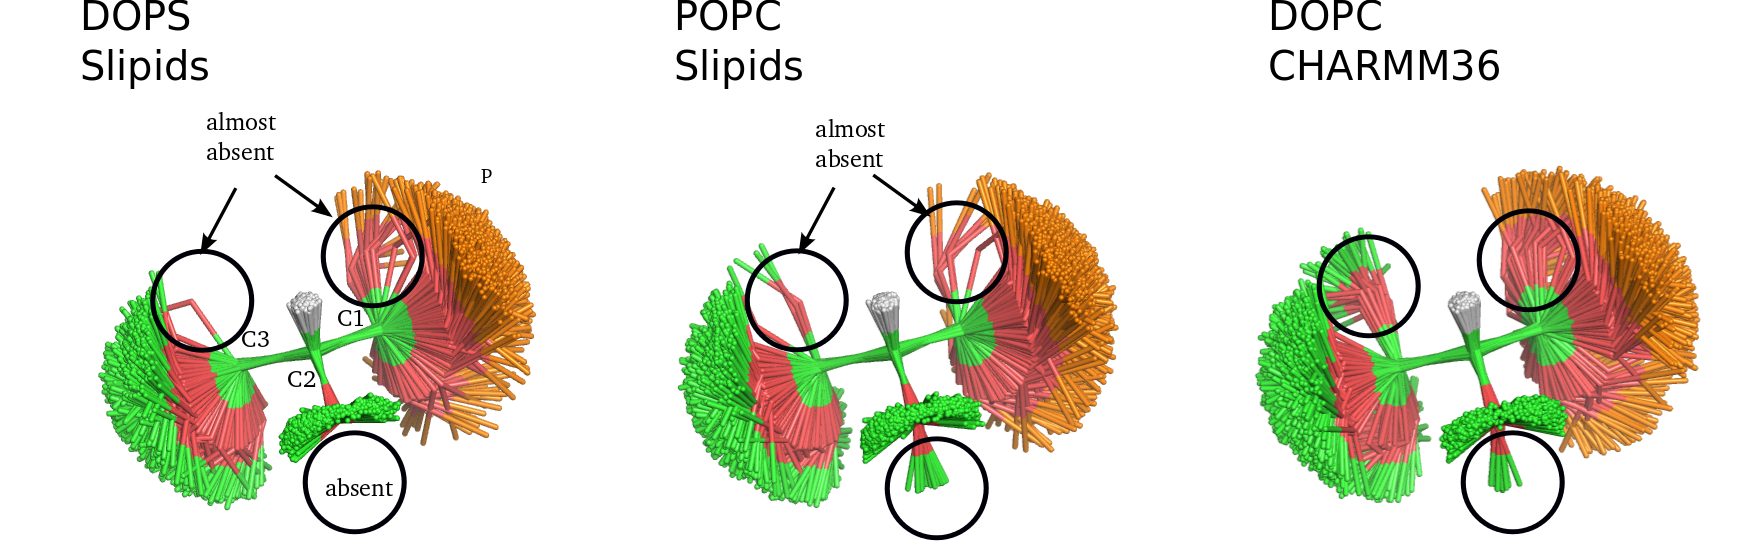
\includegraphics[width=9.0cm]{../Figs/glycerol_buslaev.png}
  \caption{\label{glycerol_buslaev}
    Snapshots overlayed from different simulations for glycerol backbone region
    by Pavel Buslaev.
  }
\end{figure}

\todo{Dihedral angle distribtions in Fig. \ref{dihedrals} should be included in the discussion.}

\subsection{Effect of PS on PC headgroup}
The headgroup order parameters of POPC 
mixed with PS lipids are shown in Fig. \ref{HGorderparametersPCvsPEPSPG}
from different simulation model and experiments \cite{scherer87} with different
mole fractions. As already discussed previosly, the PC lipid headgroup behaviour
follows the electrometer concept in experiments when mixed with other lipids, i.e., the order
parameters increase when mixed with negatively charged lipids (PS, PI, CL, PA and PG)
remains almost unchaged when mixed with neutral lipids (PE and SM) \cite{scherer87}.
This is not the case in simulation data shown in Fig. \ref{HGorderparametersPCvsPEPSPG}.
%The addition of DOPE into a POPC and DOPC bilayers significantly decreases the PC headgroup
%order parameters in simulations with OPLS compatible version of the Berger force field \cite{tieleman06}
%in contrast to experiments \cite{scherer87}. On the other hand, the increase of the PC
%headgroup order parameters in CHARMM36 simulations mixed with PS and PG lipids is significantly
%smaller than in experiments.
\begin{figure}[]
  \centering
  \includegraphics[width=8.0cm]{../Figs/HGorderparametersPCvsPS.eps}
  \caption{\label{HGorderparametersPCvsPEPSPG}
    PC headgroup order parameters from mixtures with PE, PS and PG
    lipids with various mole fractions from different simulation models and experiments \cite{scherer87}.
    Signs are determined as discussed in \cite{botan15,ollila16}.
  }
  \todo{Simulation of CHARMM36 at 298K should be maybe rerun with Gromacs 5.}
\end{figure}

\todo{More data to be collected before discussion.}

\subsection{Effect of PC on PS headgroup}
The headgroup order parameters of PS mixed with varying amounts of PC
from simulations and experiments \cite{borle85,roux90}
are shown in Fig. \ref{HGorderparametersPSPGvsPC}. The effect of increasing
amount of PC to PS headgroup seems to qualitatively incorrect in CHARMM36 simulations.
The $\beta$-carbon order parameter increases in experiment, but decreases
in simulations with both tested counterions (Na+ and K+). Larger
$\alpha$-carbon order parameter decreases with the addition of PC
in experiment, while the lower remains unchanged. In simulations the
larger increases and the lower decreases.
Interestingly, the $\alpha$-carbon order parameters are closer to experiments
in pure PS system with K+ counterions than with Na+. 
%The changes in PG headgroup order parameters are minor in simulations, which
%is in line with the only available experiment for the $\beta$-carbon.
\begin{figure}[]
  \centering
  \includegraphics[width=8.0cm]{../Figs/HGorderparametersPSvsPC.eps}
  \caption{\label{HGorderparametersPSPGvsPC}
    PS order parameters from mixtures with PC
    lipids with various mole fractions from different simulation models and experiments \cite{borle85,roux90}.
    Signs for PS are measures as described in SI.
  }
  \todo{Some simulations contain potassium as counterions, while some sodium.
    All experiments here contain some amount of sodium salt. The best
    ion concentrations for comparison should be figured out.} \\
  \todo{Why there is difference between CHARMM36 simulation results from POPS:POPC mixture and
  pure POPS? Discussion in https://github.com/NMRLipids/NMRlipidsIVotherHGs/issues/1}
\end{figure}



\subsection{Ca$^{2+}$ binding affinity in bilayers with negatively charged PS lipids}

PC lipid headgroup order parameters can used to measure ion binding
affinity, because their magnitude is proportional
to the amount of bound charge in bilayer \cite{seelig87,catte16}.
The molecular electrometer concept can be used also
for bilayers containing PC lipids mixed with charged lipids \cite{borle85,macdonald87,roux90}.
This is demonstrated in Fig. %s \ref{OrderParametersWithCaCl},
%\ref{OrderParametersWithCaClBELOW1M} and
\ref{OrderParameterCHANGESWithCaClBELOW1M},
showing the changes of PC headgroup order parameters %for PC headgroup $\alpha$ and $\beta$ carbons
as a function of CaCl$_2$ concentration in the presence of different amounts of
negatively charged PS or PG lipids.
%\begin{figure}[]
%  \centering
%  \includegraphics[width=9.0cm]{../Figs/LIPIDSwithCaCl.eps}
%  \caption{\label{OrderParametersWithCaCl}
%    PC headgroup order parameters as a function of CaCl concentration from experiments containing charged lipids.
%    Pure DPPC data from \cite{akutsu81}, pure POPC data from \cite{altenbach84}, 
%    POPC:POPS mixture data from \cite{roux90}, POPC:POPG mixture data with 0.1M NaCl from \cite{macdonald87}
%    and POPC:POPG mixture data without NaCl from \cite{borle85}.
%  }
%  \todo{Check the NaCl concentrations in the samples.}
%\end{figure}
%\begin{figure}[]
%  \centering
%  \includegraphics[width=9.0cm]{../Figs/LIPIDSwithCaClBELOW1M.eps}
%  \caption{\label{OrderParametersWithCaClBELOW1M}
%    Figure \ref{OrderParametersWithCaCl} zoomed to smaller concentrations.
%  }
%\end{figure}
\begin{figure}[]
  \centering
  \includegraphics[width=9.0cm]{../Figs/CHANGESwithCaCl.eps}
  \caption{\label{OrderParameterCHANGESWithCaClBELOW1M}
    The change of PC headgroup order parameters
    in the presence of different amount of negatively charged lipids
    respect to the values without added CaCl$_2$.
    The original data is the same as in Fig. \ref{OrderParametersWithCaCl}. 
  }
\end{figure}
%PC headgroup order parameters increase when negatively charged
%PS or PG are added to PC bilayer in the absense of added CaCl$_2$,
%as expected based on electrometer concept \cite{seelig87}
%(see Fig. \ref{OrderParametersWithCaClBELOW1M}).
%In electrometer concept this is explained by the tilting of
%headgroup more parallel to membrane normal \cite{??}.
The decrease of order parameters with CaCl$_2$
is more pronounced for systems with more
negatively charged lipids.% (see Fig. \ref{OrderParameterCHANGESWithCaClBELOW1M}).
Order parameters reach the values of pure PC bilayer close to CaCl$_2$ concentrations of $\sim$ 50-300mM.
At this point the Ca2+ binding presumably fully cancels the charge from negative lipids and
overcharging occurs above these concenterations.
The interpretation of this data and some other results has been that \cite{seelig90}
\begin{displayquote}
  {\it ''(i) Ca$^{2+}$ binds to neutral lipids (phosphatidylcholine, phosphatidylethanolamine) and negatively charged lipids
    (phosphatidylglycerol) with approximately the same binding constant of K = 10-20 M$^{-1}$; \\
    (ii) the free Ca$^{2+}$
    concentration at the membrane interface is distinctly enhanced if the membrane carries a negative surface
    charge, either due to protein or to lipid; \\
    (iii) increased inter-facial Ca$^{2+}$ also means increased amounts
    of bound Ca$^{2+}$ at neutral and charged lipids; \\
    (iv) the actual binding step can be described by a Langmuir
    adsorption isotherm with a 1 lipid:1 Ca$^{2+}$ stoichiometry, provided the interfacial concentration C$_M$, is
    used to describe the chemical binding equilibrium.''}
\end{displayquote}

\todo{When we have more data for Ca binding to PS containing bilayers, the discussion will be updated and PG results moved
to other manuscript.}
Comparison of Ca$2+$ binding in PG between CHARMM36 simulations and experiments \cite{borle85}
is shown in Fig. \ref{changesWITHCaClPG}. The decrease of $\alpha$ order parameter
is in agreement with experiments, while decerase of $\beta$ order parameter is overestimated.
The result is very similar to the results with PC in NMRlipids II publication \cite{catte16}.
It should be, however, noted that the $\beta$-order parameters are not actually measured for PG,
but they are calculated from empirical relation $\Delta S_{\beta}=0.43\Delta S_{\alpha}$ \cite{akutsu81}.
Anyway, the data presented in NMRlipids II project and in Fig. \ref{changesWITHCaClPG} together
suggest that Calcium binding is similarly overestimated by CHARMM36 model in pure POPC bilayers and mixtures with
POPG. The good agreement of $\alpha$ carbon would be explained by too weak dependence of its order
parameter of bound charge
\todo{The response of CHARMM36 against cationic surfactant experiments \cite{scherer89} is to be checked.
  I have already ran the simulations, analysis yet to be done}.
\begin{figure}[]
  \centering
  \includegraphics[width=9.0cm]{../Figs/CHANGESwithCaClPGPS.eps}
  \caption{\label{changesWITHCaClPG}
    PG order parameters as a function CaCl$_2$ concentration from experiments \cite{borle85} and CHARMM36 simulations.
    Note that beta order parameter is calculated from empirical relation $\Delta S_{\beta}=0.43\Delta S_{\alpha}$ \cite{akutsu81}, not actually measured. 
  }
\end{figure}

Also dependence of $\beta$-carbon of PG on CaCl$_2$ concentration is compared with
experiments \cite{borle85} in Fig. \ref{PSPGchangesWITHCaCl}. Absolute value of
the order parameter is too large without ions, but rapid decrease due to addition of
CaCl$_2$ is observed in agreement with experiments for systems with 1:1 mixture of POPC and POPG.
In addition, absolute value in systems with CaCl$_2$ is in agreement with experiments.
However, system with 4:1 mixture of POPC and POPG behaves differently, but experimental
data is not available for comparison for this mixture.

\todo{More simulation data for systems with negatively charged lipids and CaCl$_2$ to be collected}

\subsection{Effect of Ca$2+$ binding to PS headgroup}

Also the experimental order parameters for PS and PG headgroups
as a function of CaCl$_2$ concentration are shown in Fig. \ref{PSPGchangesWITHCaCl}.
\todo{These should be compared to simulations for potential structural interpretation of the changes.}
\begin{figure}[]
  \centering
  \includegraphics[width=9.0cm]{../Figs/PSPGwithCaCl.eps}
  \caption{\label{PSPGchangesWITHCaCl}
    PG and PS order parameters a function CaCl$_2$ concentration taken from \cite{borle85} and \cite{roux90}, respectively.
  }
  \todo{Get the small concentration data from the inserts}
\end{figure}





\section{Conclusions}


% Tables may be be put in the text as floats.
% Here is an example of the general form of a table:
% Fill in the caption in the braces of the \caption{} command. Put the label
% that you will use with \ref{} command in the braces of the \label{} command.
% Insert the column specifiers (l, r, c, d, etc.) in the empty braces of the
% \begin{tabular}{} command.
%
% \begin{table}
% \caption{\label{} }
% \begin{tabular}{}
% \end{tabular}
% \end{table}

% If you have acknowledgments, this puts in the proper section head.
\begin{acknowledgments}
% Put your acknowledgments here.
\end{acknowledgments}
\newpage
\appendix
\begin{center}
{\bf SUPPLEMENTARY INFORMATION}
\end{center}

\section{Simulated systems}
\begin{table*}[!p]
%\begin{sidewaystable*}[!p]
\centering
\caption{List of MD simulations. The salt concentrations calculated as 
   [salt]=N$_{\rm c} \times$[water]\,/\,N$_{\rm w}$, where [water]\,=\,55.5~M.
%   these correspond the concentrations reported in the experiments by Akutsu et al.~\cite{akutsu81}.
%   The lipid force fields named as in our previous work~\cite{botan15}.
}\label{IONsystems}
\begin{minipage}[t]{\textwidth}
\begin{tabular}{l c c r r r r r r c c}
  %\hline
  % some footnotes are not visible in typeset-MS (pdf)
 lipid/counter-ions & force field for lipids / ions & NaCl (mM) & CaCl$_2$\,(mM) &  \footnote{Number of lipid molecules with largest mole fraction}N$_{\rm l}$   &  \footnote{Number of water molecules}N$_{\rm w}$   & \footnote{Number of additional cations}N$_{\rm c}$  & \footnote{Simulation temperature}T (K)  & \footnote{Total simulation time}t$_{{\rm sim}}$(ns) & \footnote{Time used for analysis}t$_{{\rm anal}}$ (ns) &   \footnote{Reference for simulation files}files\\
  \hline
  DPPE  & Slipids \cite{jambeck12b} &0 & 0        & 288 			   		& 9386 & 0  & 336  & 200 & 100 & \cite{slipidsDPPEfiles}  \\
    \hline
    DOPS/Na$^+$  & CHARMM36 \cite{??}  \todoi{Correct citation for CHARMM DOPS}      &0 & 0        & 128 			   		& 4480 & 0  & 303  & 500 & 100 & \cite{??}
    \todoi{By Piggot: http://nmrlipids.blogspot.com/2017/03/nmrlipids-iv-headgroup-glycerol.html?showComment=1491425687561\#c4932902612512697301. We need to decide the switching version or discuss this somehow.}  \\
    DOPS/Na$^+$  & CHARMM36ua \cite{??} \todoi{Correct citation for CHARMMua DOPS}        &0 & 0        & 128 			   		& 4480 & 0  & 303  & 500 & 100 & \cite{??}
    \todoi{Delivered by Piggot. We need to decide the switching version or discuss this somehow. Data to be uploaded in Zenodo?}  \\
    DOPS/Na$^+$  & Slipids \cite{jambeck13}        &0 & 0        & 128 			   		& 4480 & 0  & 303  & 500 & 100 & \cite{??}
    \todoi{Delivered by Piggot. We need to decide the cut-off version or discuss this somehow. Data to be uploaded in Zenodo?}  \\
    DOPS/Na$^+$  & Slipids \cite{jambeck13}        &0 & 0        & 288 			   		& 11232 & 0  & 303  & 200 & 100 & \cite{slipidsDOPSfiles} \\
    DOPS/Na$^+$  & Berger \cite{mukhopadhyay04}        &0 & 0        & 128 			   		& 4480 & 0  & 303  & 500 & 100 & \cite{??}
    \todoi{Delivered by Piggot. Data to be uploaded in Zenodo?}  \\
    DOPS/Na$^+$  & GROMOS-CKP \cite{??} \todoi{Correct citation(s) for CKP.}       &0 & 0        & 128 			   		& 4480 & 0  & 303  & 500 & 100 & \cite{??}
    \todoi{Delivered by Piggot. We need to decide between RF and PME or discuss this somehow. Data to be uploaded in Zenodo?}  \\
    \hline
    POPS/Na$^+$  & CHARMM36 \cite{??} \todoi{Correct citation for CHARMM POPS}        &0 & 0        & 128 			   		& 4480 & 0  & 298  & 500 & 100 & \cite{??}
    \todoi{Delivered by Piggot. We need to decide the switching version or discuss this somehow. Data to be uploaded in Zenodo?}  \\
    POPS/Na$^+$  & CHARMM36ua \cite{??} \todoi{Correct citation for CHARMMua DOPS}        &0 & 0        & 128 			   		& 4480 & 0  & 298  & 500 & 100 & \cite{??}
    \todoi{Delivered by Piggot. We need to decide the switching version or discuss this somehow. Data to be uploaded in Zenodo?}  \\
    POPS/Na$^+$  & Slipids \cite{jambeck13}        &0 & 0        & 128 			   		& 4480 & 0  & 298  & 500 & 100 & \cite{??}
    \todoi{Delivered by Piggot. We need to decide the cut-off version or discuss this somehow. Data to be uploaded in Zenodo?}  \\
    \hline
    POPC:POPS (5:1)/Na$^+$  & CHARMM36 \cite{klauda10,??} \todoi{Correct citation for CHARMM POPS}        &0 & 0        & ? 			   		& ? & 0  & ?  & ? & ? & \cite{??}
    \todoi{Details to be filled and data to be uploaded in Zenodo by Ollila.}  \\
    \hline
    POPG/Na$^+$  & CHARMM36 \cite{??} \todoi{Correct citation for CHARMM POPG}        &0 & 0        & ? 			   		& ? & 0  & ?  & ? & ? & \cite{??}
    \todoi{Details to be filled and data to be uploaded in Zenodo by Ollila.}  \\
    POPG/Na$^+$  & Slipids \cite{jambeck13}     &0 & 0        & 288 			   		& 10664 & 0  & 298  & 250 & 100 & \cite{slipidsPOPGfiles} \\
    \hline
    DPPG/Na$^+$  & Slipids \cite{jambeck13}     &0 & 0        & 288 			   		& 11232 & 0  & 314  & 200 & 100 & \cite{slipidsDPPGfiles} \\
    DPPG/Na$^+$  & Slipids \cite{jambeck13}     &0 & 0        & 288 			   		& 11232 & 0  & 298  & 400 & 100 & \cite{slipidsDPPGfilesT298K} \\
\end{tabular}
\end{minipage}
%\end{sidewaystable*} 
\end{table*}


\section{Measurements of order parameter sign}

Fig. \ref{PShgSIGNS} summarizes the experimental results on the order parameter sign
measurement for POPS sample. The experimental protocol is the same used in Ref. \citenum{ferreira16}.
In (a) you see the headgroup region of the INEPT spectrum where alpha and beta are
identified. In (b) you have the R-PDLF slices for alpha and beta where you see one single
splitting for beta (which gives an order parameter equal to 0.12), and for alpha a superposition
of a large splitting (order parameter equal to 0.09) and a very small splitting which cannot be
calculated. On the bottom you have the S-DROSS slices of these two carbons. The grey lines show a
random collection of slices from noise such that it gets clear what is significant. The S-DROSS
slice for beta clearly shows that the order parameter is negative. The slice for alpha shows that
the higher order parameter is positive and suggests that the smaller order parameter is negative
(from the deviation towards negative values in the longer t1 times).
\begin{figure}[]
  \centering
  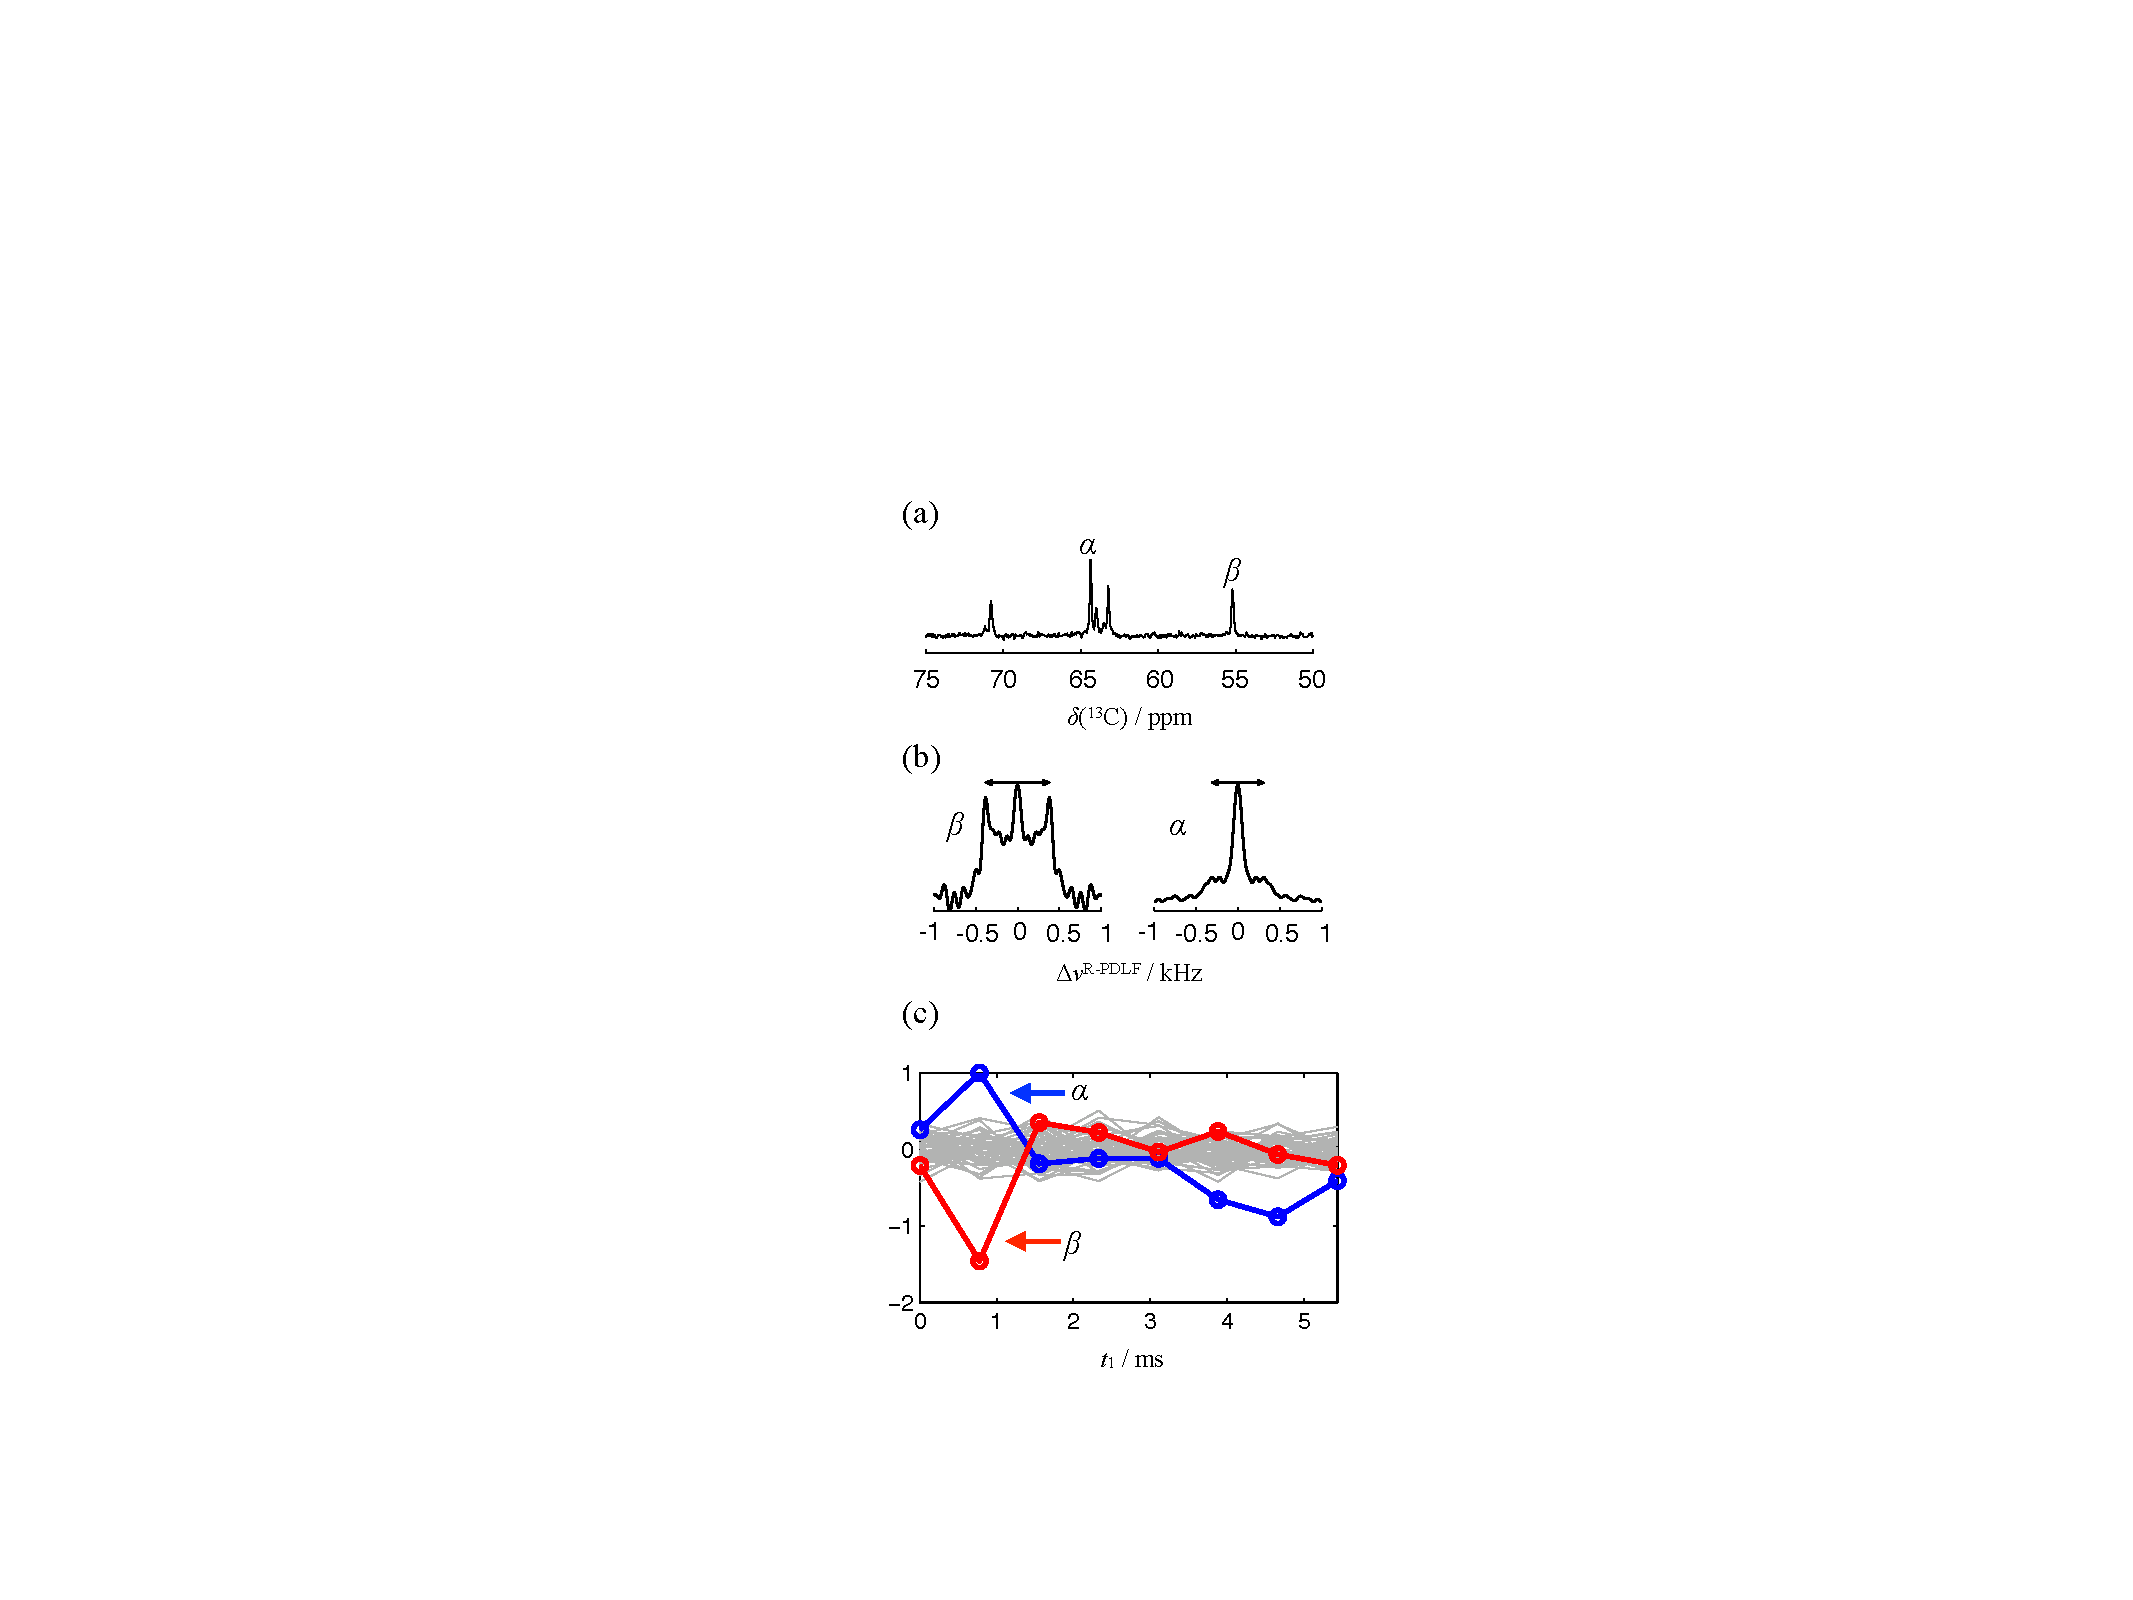
\includegraphics[width=9.0cm]{../Figs/PShgSIGNS.pdf}
  \caption{\label{PShgSIGNS}
    Experimental results for sign measurement for POPS sample
  }
\end{figure}

The results updated with SIMPSON simulations for the SDROSS profiles
are shown in Fig. \ref{PShgSIGNSsimpson}. The value for the smaller
alpha order parameter is taken from Fig 3 in Ref. \citenum{roux91},
because resolution in 13C NMR experiments was nor high enough to determine
numerical value for this. The plots in Fig. \ref{PShgSIGNSsimpson} (c) show
the following. The error bars and points are the experimental SDROSS data.
The thick lines are SIMPSON simulations. The simulations were done by using
the order parameter for beta equal to -0.12 and for alpha one order parameter
equal to 0.09 and the other equal to -0.02 (black) or 0.02 (grey).
Since the black lines agree with experimental data, we conlude that
the order parameters for $\beta$ carbon are -0.12 and for $\alpha$
order parameters are 0.09 and -0.02.
\begin{figure}[]
  \centering
  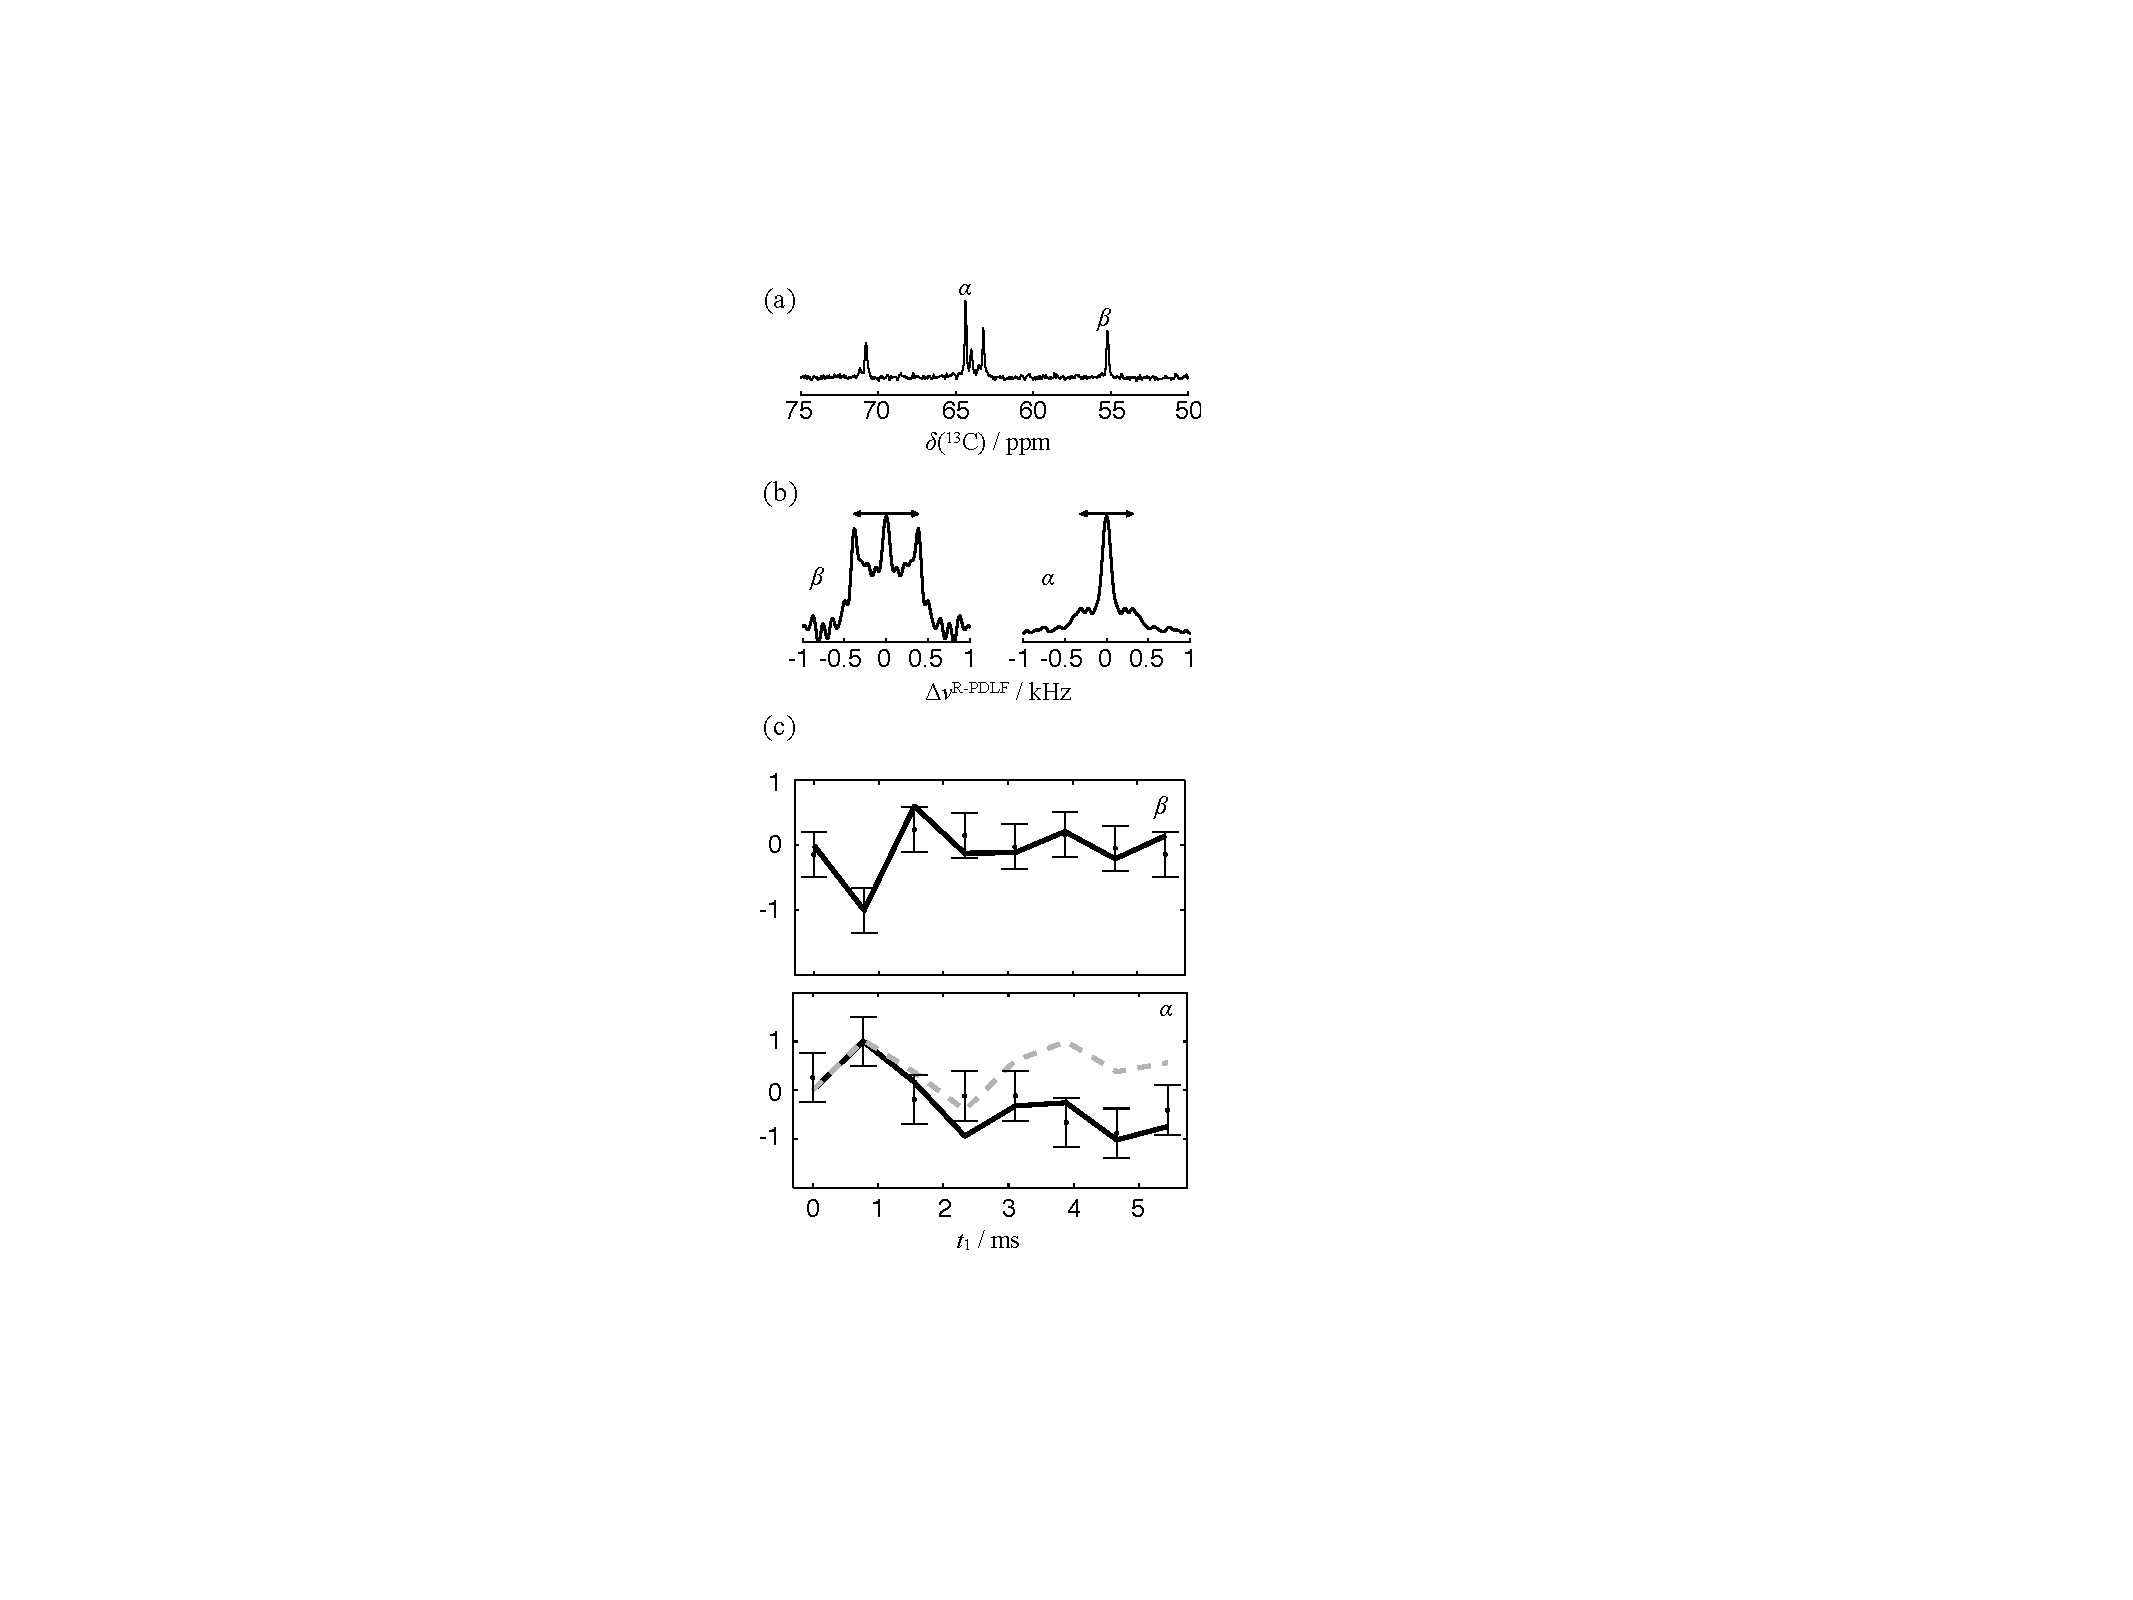
\includegraphics[width=9.0cm]{../Figs/PShgSIGNSsimpson.pdf}
  \caption{\label{PShgSIGNSsimpson}
    Experimental results for sign measurement for POPS sample
  }
\end{figure}

\section{Dihedrals}
\begin{figure*}[]
  \centering
  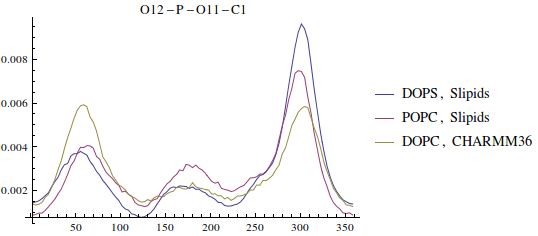
\includegraphics[width=8.0cm]{../Figs/dihed1.png}
  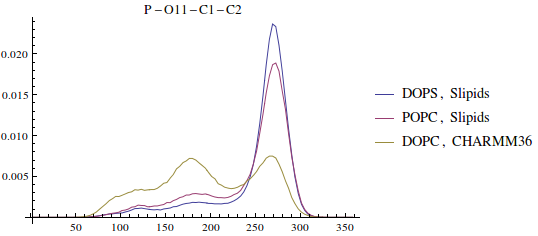
\includegraphics[width=8.0cm]{../Figs/dihed2.png}
  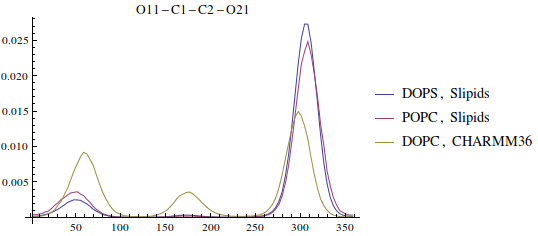
\includegraphics[width=8.0cm]{../Figs/dihed3.png}
  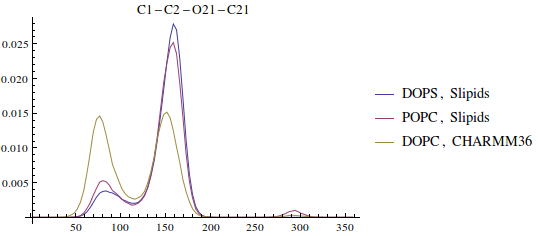
\includegraphics[width=8.0cm]{../Figs/dihed4.png}
  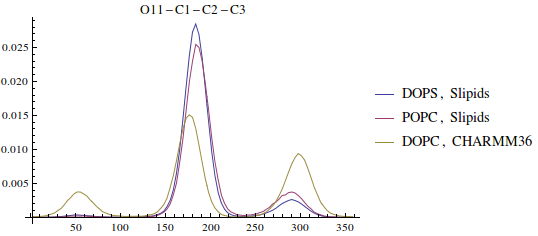
\includegraphics[width=8.0cm]{../Figs/dihed5.png}
  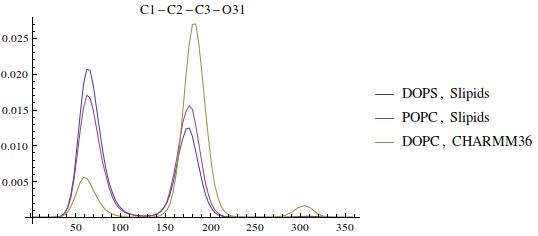
\includegraphics[width=8.0cm]{../Figs/dihed6.png}
  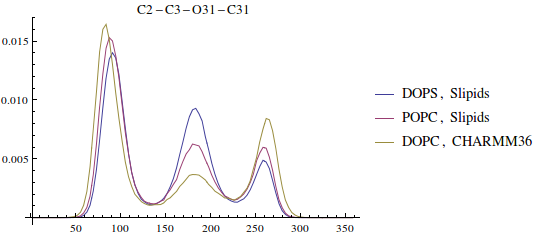
\includegraphics[width=8.0cm]{../Figs/dihed7.png}
  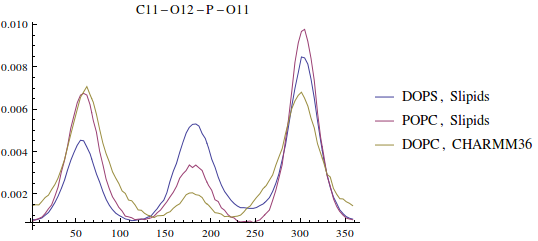
\includegraphics[width=8.0cm]{../Figs/dihed8.png}
  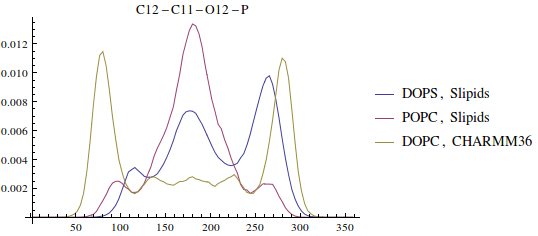
\includegraphics[width=8.0cm]{../Figs/dihed9.png}
  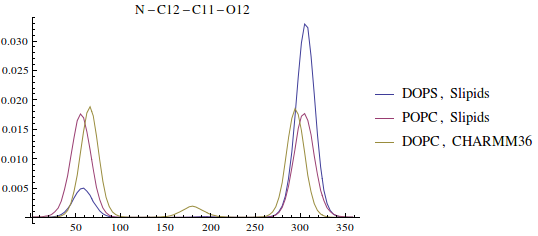
\includegraphics[width=8.0cm]{../Figs/dihed10.png}
  \caption{\label{dihedrals}
    Experimental results for sign measurement for POPS sample
  }
\end{figure*}

% Create the reference section using BibTe
\bibliography{refs.bib}

%\newpage
%\section{APPENDIX: The NMR results reported by Tiago Ferreira}

\listoftodos

\end{document}
%
% ****** End of file aiptemplate.tex ******
